As indicated in \figref{Fig:Overview}, we build upon the \mcsaf framework by
adding taming transformations and by producing a more specialized Tame IR.
The \mcsaf framework provides us with a three-address form of the AST, reducing many
complicated \matlab constructs. We further reduce the AST to build
the Tame IR. The main contributions of the Tame IR, beyond the
three address form previously provided by \mcsaf are:

\begin{itemize}
\item Rather than providing a reduced form of the AST, as provided
by \mcsaf, we implement the Tame IR as a complete set of new
nodes. The interfaces of these nodes enforce the constraints of the IR.
\item The Tame IR reduces the total number of possible
AST nodes. In particular, we remove all expression nodes, and express
their operations in terms of statements and function calls.
\item The Tame IR reduces some complexity of \matlab. Some
of these reductions would not have been possible to be provided
by the \mcsaf framework, because it is completely semantics
preserving. Because the tamer framework does impose constraints
on \matlab to make it amenable to static compilation, it
is possible to further reduce the AST in ways that is
not possible with semantics-preserving transformations. In particular, we
simplify lambda expressions and remove switch statements;
we also place all comments into empty statements, rather
than have them annotated to statement nodes.
\item The Tame IR specialize nodes according to their semantics,
and provides nodes that signify the operation performed.
\item The Tame IR provides information that is not available in 
the AST. In particular, it separates functions and variables,
utilizing the kind analysis \cite{KindAnalysis}.
\end{itemize}

Rather than implementing completely new nodes, all Tame IR nodes are
extensions of existing AST nodes. This means that any Tame IR program
tree is a valid AST as well. A program in the Tame IR is also a
valid \matlab program, with one exception, which is discussed
in \secref{sec:assignStmts}. This difference is removed when the Tame
is pretty printed, which will produce valid \matlab again.

The intention of the Tame IR is to make it easier to implement
analyses, by reducing the number of nodes, by specializing nodes to
signify their operation, and by providing some static information. By
keeping the Tame IR an almost valid AST, any analysis written for the
AST should work for the Tame IR as well; by keeping it valid \matlab
(at least when pretty printed), it should be easier to debug analyses
and transformations. One goal for our overall Taming framework is to
produce an IR whose operations are low-level enough to map fairly
naturally to static languages like {\sc FORTRAN}.

Besides providing the IR nodes and the transformations to 
build the Tame IR, we have also extended the visitor classes and
flow analyses of the \mcsaf framework so that it can be used
to implement flow analyses that explicitly use the IR.

In the following sections we first introduce the Tame IR and its nodes,
and then provide an overview of some of the transformations used to
arrive at the Tame IR.


\section{The Tame IR}
The Tame IR consists of nodes that extend existing AST nodes.
Some of these nodes extend the AST and merely enforce 
constraints that correspond to the three-address form
semantics of the Tame IR. Some nodes are extensions of
the AST nodes that do not change the interface at all,
they merely exist to complete the Tame IR, so that
a program may consist only of IR Statements.

For assignment nodes, however, we provide several specializations
that correspond to many different operations that can be
performed by an assignment statement. The AST only provides
a single assignment statement with an expression on the lhs
and rhs. This is what the three-address form of \mcsaf
provides as well, even when the three-address transformations
will have reduced the actual structure of an assignment.

%Since a Tame IR node extends and represents valid AST nodes, it is possible
%for a Tame IR node to contain other AST nodes. The Tame IR provides
%interfaces to access information about the IR nodes, but it 
%is also possible to access and change internal AST nodes
%using the AST interfaces. This may lead to undefined behavior.

In the following sections, we present all the Nodes of the Tame IR.
A complete grammar is given in appendix \appendixref{chap:irgrammar}.


\subsection{Assignment Statements}
\label{sec:assignStmts}
%McSAF will only allow one complex expression on either the lhs or rhs, and
%that complex expression can not contain other complex expressions.
For the Tame IR, we have extended the AST's assignment statement into 
several specialized versions, as seen in 
\figref{Fig:assign}. These all represent different operations
in terms of assignment statements. Note in particular that we have
different nodes for the syntactically identical array accesses and
calls, given that the Tame IR differentiates between them, unlike the
AST.  In the following we describe all the different kinds of
extensions of the assignment statement that are part of the Tame IR.

\begin{figure}[htbp]
\begin{center}
\includegraphics[width=6.2in]{Figures/assign.eps}
\caption{Specializations of an assignment statement}
\label{Fig:assign}
\end{center}
\end{figure}

% new command to put indented lstinlines, with a preceding newline
\DeclareRobustCommand{\lstd}[1]{\\ \phantom{.} \hspace{1cm} \lstinline{#1}} 


\begin{description}
%- abstract assignments
\item[TIRAbstractAssignStmt] \hfill \\
An abstract class representing all assignment nodes of the Tame IR. This class
extends the AST node {\tt AssignStmt}. The analysis framework allows
specifying flow equations for every node, including all the abstract nodes.

\vspace{.5cm}
\item[TIRAbstractAssignFromVarStmt] \hfill \\
Assignments from variables are of the form
\lstd{... = x}\\
i.e. they have a rhs which is a name referring to a variable.
This is an abstract node class representing the following nodes:

\begin{description}
\item[TIRArraySetStmt, TIRDotSetStmt, TIRCellArraySetStmt] \hfill \\
The `set'-assignments represent AssignFromVarStmts whose lhs are indexing operations, i.e.
they represent assignment indexing operations that correspond to the \matlab builtin
function {\tt subsasgn}. For example, they represent the following operations:
\lstd{ a(i,j) = x, a.s = x, a\{i,j\} = x}
\end{description}


\vspace{.5cm}
\item[TIRAbstractAssignToListStmt] \hfill \\
Assignments to lists are assignments with multiple possible
target variables. I.e. they are assignments of the form
\lstd{[v1, v2, v3, ... , vn] = ...}

Within the Tame IR, it is allowed that the list of result variables
is empty, which is not valid in \matlab. This is the only deviation
of the Tame IR from being valid \matlab (the AST does not enforce
this restriction). Empty lhs lists are used
to represent expression statements. For example, within the Tame
IR, a statement like
\lstd{foo(3);}

is represented as
\lstd{[] = foo(3);}\\
This allows us to represent all expressions in terms
of statements, while having IR nodes that are merely extended
AST nodes (in this case {\tt AssignmentStmt}),
while also not having multiple versions for statements, either
as assignment or expression statements.\\
When pretty-printed, an assignment with an empty lhs list will
return an expression statement.\\

\begin{description}
\item[TIRArrayGetStmt, TIRCellArrayGetStmt, TIRDotGetStmt] \hfill \\
The `get'-assignments are assignments to lists that are represented
by the \matlab builtin function {\tt subsref}, i.e. they have
indexing operations on the rhs.
Note that structure-referencing and cell-indexing may result
in multiple return values that can be assigned, while
array-indexing produces only one value. However, array-indexing
is also used when calling a value of mclass {\tt function\_handle}.
In that case, the referenced function gets called, possibly
resulting in multiple return values. When any of the above operations
is overloaded, the operation may also result in multiple return values.

\item[TIRCallStmt] \hfill \\
Calls are assignments of the form
\lstd{[r1, r2, ... , rn] = f(a1, a2, ..., an);}

Where $r_i$ and $a_i$ are variables. Note the similarity to the
array-get statement. The difference is that $f$ is a name
that has to refer to a function.
\end{description}

\vspace{.5cm}
\item[TIRAbstractAssignToVarStmt] \hfill \\
These represent assignments of the form,
\lstd{x = ...}

There is a name on the lhs representing a single variable. 
These are used for assignments where there always is exactly
one variable on the lhs. This makes them simpler to analyze
than the assignments to lists, because there don't need to be
any checks for the existence of enough target variables, etc.
\begin{description}
\item[TIRAssignLiteralStmt] \hfill \\
Literal assignments are used to assign numerical and string
literals to a variable, i.e. they may be used to represent
the following statements:
\lstd{x = 3, x = 'hi'}\\
In \rednote{ \matlab, {\tt true}} and {\tt false} are not literals, but builtin
functions. These functions actually allow arguments specifying matrix
dimensions to produce logical matrices.\\
The assign-literal statements are the only place in the
Tame IR where literals may occur; other statements
usually operate on just variables.\\

\vspace{.2cm}
\item[TIRCreateFunctionHandleStmt] \hfill \\
These assign-to-var statements allow the creation of function handles,
either creating function pointers, or by creating an anonymous 
function using lambda. They are thus of the form
\lstd{t = @f;}   

 or            
\lstd{t = @(x1,x2,...) f(a1,a2,..,an,x1,x2,...);}

where $f$ is a name referring to a function. The variables $a_i$ through
$a_n$ encapsulate workspace variables within the anonymous function,
there may be 0 or more of such variables. The transformation
from arbitrary lambda expressions to statements of the above form
is discussed in detail in \secref{sec:lsimp}.

\item[TIRCopyStmt] \hfill \\
Copies are assignments of the form
\lstd{x = y;}

where $x$ and $y$ are names referring to variables.
\end{description}
\end{description}

\subsection{Control Flow Statements}
\begin{description}
\item[TIRIfStmt, TIRWhileStmt] \hfill \\
The if and while statements in the Tame IR are almost the same
as the corresponding statements in the AST. The only constraint,
being a three-address form, is that the condition-expressions
have to be names referring to variables.

\item[TIRForStmt] \hfill \\
The for statement in the Tame IR is of the form
\lstd{for i = low:inc:hi}
\lstd{  ...}
\lstd{end}

where $i$, $low$, $inc$ and $hi$ are names referring to variables. $inc$
is optional.

\item[TIRReturnStmt, TIRBreakStmt, TIRContinueStmt] \hfill \\
These control flow statements are the same as their AST counterparts.
\end{description}

\subsection{Other Statements}
\begin{description}
\item[TIRGlobalStmt, TIRPersistentSmt] \hfill \\
These statements allow declaring variables to be global or persistent.
The Tame IR imposes the constraint on \matlab that no variable
may be used before a global definition. \matlab merely issues a warning
in this case. \matlab does not allow using a persistent variable
before the declaration.

\item[TIRCommentStmt] \hfill \\
In the AST, comments are annotated to AST-nodes. When replacing
AST nodes with other AST nodes, one would thus have to ensure that comments are copied
as well. In order to make transformations of the tree easier,
we have opted to place all comments into empty statements, so 
that no other statement may have annotated comments.

\end{description}

\subsection{Non-Statement Nodes}
Besides all the above statement nodes, the Tame IR includes the following
nodes which are not statements.

\begin{description}
\item[TIRNode, TIRStmt] \hfill \\
These are interfaces. Any Tame IR node implements {\tt TIRNode}.
Any Statement of the Tame IR implements {\tt TIRStmt}.

\item[TIRFunction] \hfill \\
{\tt TIRFunction} is an extension of the function node of the AST.  It
ensures that all statements inside the body are {\tt TIRStmt} nodes.
The functions also include information that is not readily available to AST
function nodes, namely a simple symbol table separating names into
functions and variables (the result of the kind analysis).  It also
provides the list of global and persistent variables declared inside
the function body.

\item[TIRStatementList] \hfill \\
A simple extension of the {\tt StatementList} that is part of the AST,
to ensure that all elements are {\tt TIRStmt} nodes.

\item[TIRCommaSeparatedList] \hfill \\
Used as a list of names for arguments to calls, and for indices of
indexing operations, and targets in list-assignments. Besides names,
indexing operations may include a colon (:), for example as used in
the indexing operation
\lstd{a(:,3)}

Here, {\tt :,3} would be represented as a comma-separated list.

As more of the \matlab language is supported, more possible elements
may get added, for example \matlab's tilde expression `\texttildelow', which allows
discarding results of calls.


\end{description}

%\newpage
\section{Tame IR Transformations}

The Tame IR of an AST is built by transforming the three-address form
produced by the \mcsaf framework. Given this three-address form, most
of the transformations produce equivalent nodes of the IR, merely checking
constraints. To transform an incoming assignment statement,
the transformations have to check what kind of assignment it is,
and produce the appropriate IR assignment. All these transformations
do not actually transform the underlying \matlab code, they merely
change the representation of it.

Besides these node-representation transformations, the Tame IR transformations
also include some transformations that actually change the underlying
\matlab code. These are presented below. Note how some of these transformations
impose slight constraints on the \matlab code, which are thus part of the 
Tame \matlab language subset.


\newpage
\subsection{Reduction of Operations to Calls}

The Tame IR has no operators. In order to transform to the Tame IR, all operators
have to be transformed into calls to equivalent builtin functions.
Note that users may already be using builtin functions rather than operators, so
after the transformation, all operations are expressed in the same way.
The list of operators thus transformed in presented in \tableref{Fig:opTables}.

The missing short circuit logical operations ({\tt \&\&} and {\tt ||}) are already reduced by the
\mcsaf framework into equivalent if-then-else statements.

The transformation does not reduce the indexing operators '{\tt ()}',
'{\tt \{\}}' and '{\tt .}'.  They do correspond to the builtin
functions {\tt subsref} and {\tt subsasgn}, for indexing operations on the
rhs and lhs, respectively. Note, however, that \matlab uses the same
indexing operator for all indexing operations.  Consequently, \matlab
internally has to add arguments to specify the exact indexing
operation used. This information is stored in a structure. 
For example, an indexing operation like
\vspace{-.5cm}
\begin{lstlisting}
x = a(i,j);
\end{lstlisting}
May look like the following, if {\tt subsref} was used explicitly:
\vspace{-.5cm}
\begin{lstlisting}
s.type = '()';
s.subs = {i,j};
x = subsref(a,s);
\end{lstlisting}
Note the structure that contains the type of indexing (as a string),
and the indices, which are themselves stored as a cell array.
If the Tame IR reduced indexing operators, it would actually generate
more complex code, which may be harder to analyze.

\begin{figure}[htbp]
\begin{center}
\begin{tabular}{p{2.2in} p{3in}}
\begin{lstlisting}
   x = a + b
\end{lstlisting}
&
\begin{lstlisting}
   x = plus(a,b)
\end{lstlisting}
\\
(a) operation & (b) equivalent call 
\end{tabular}
\caption{Transforming operations to calls } \label{Fig:Lambda}
\end{center}
\end{figure}


With this in mind, analyses have to be aware that it is possible not only to
overload calls to functions, but also indexing operations. An accurate
analysis thus has to check for overloaded functions for calls, as well
as all `get'-assignments and all `set'-assignments.


After the operator reduction, analyses written for the Tame IR should
utilize the builtin framework.  That is, analysis writers should
provide a flow analysis of the AST nodes using the \mcsaf analysis
framework, and flow equations for builtins using the builtin
framework.  This simplifies the flow analysis of the AST nodes
themselves, because there are fewer nodes, and helps separating 
the definition of the flow equations of the AST-nodes
from
the definition of flow equations for builtin operations and functions.



\begin{table}[htbp]
\begin{center}
\begin{tabular}{c c c}
\begin{tabular}{c}
binary numerical operators \\
\begin{tabular}{|c|c|} \hline
{\tt + } & {\tt plus } \\       \hline
{\tt -  } & {\tt minus } \\ \hline

{\tt *  } & {\tt mtimes } \\ \hline
{\tt /  } & {\tt mrdivide } \\ \hline
{\tt \verb|\|  } & {\tt mldivide } \\ \hline
{\tt \verb|^| } & {\tt mpower } \\ \hline

{\tt .*  } & {\tt times } \\ \hline
{\tt ./  } & {\tt rdivide } \\ \hline
{\tt .\  } & {\tt ldivide } \\ \hline
{\tt .\verb|^|  } & {\tt power } \\ \hline
\end{tabular}
\end{tabular}
&
\begin{tabular}{c}
other binary operators\\
\begin{tabular}{|c|c|} \hline
{\tt \&  } & {\tt and } \\ \hline
{\tt |  } & {\tt or } \\ \hline

{\tt <  } & {\tt lt } \\ \hline
{\tt >  } & {\tt gt } \\ \hline
{\tt <=  } & {\tt le } \\ \hline
{\tt >=  } & {\tt ge } \\ \hline
{\tt ==  } & {\tt eq } \\ \hline
{\tt ~=  } & {\tt ne } \\ \hline
\end{tabular}
\end{tabular}
&
\begin{tabular}{c}
unary operators\\
\begin{tabular}{|c|c|} \hline
{\tt -  } & {\tt uminus } \\ \hline
{\tt + } & {\tt uplus } \\ \hline
{\tt .\textquotesingle  } & {\tt transpose } \\ \hline
{\tt \textquotesingle  } & {\tt ctranspose } \\ \hline
{\tt \texttildelow  } & {\tt not } \\ \hline
\end{tabular}
\\
\\
colon\\
\begin{tabular}{|c|c|} \hline
{\tt :  } & {\tt colon } \\ \hline
{\tt : :  } & {\tt colon } \\ \hline
\end{tabular}
\end{tabular}

\end{tabular}
\end{center}
\caption{\matlab operators and their corresponding builtin functions.}
\label{Fig:opTables}
\end{table}



\newpage
\section{Lambda Simplification}
\label{sec:lsimp}

\matlab supports lambda expressions. In order to be compatible with the Tame
IR, their bodies  need to be converted to a three address form in some way.
\matlab lambda expressions are single expression (rather than, say,
statement lists), that the \mcsaf framework leaves intact in their
 original form, due to the difficulty of reducing a lambda expression
 while still maintaining the full
\matlab semantics.
For the Tame IR we extract the body of the lambda expression into an
external function. The lambda expression still remains, but will encapsulate
only a single call, all whose arguments are variables.  For example, the lambda
simplification will transform the expression in \figref{Fig:Lambda}(a) to the
code in \figref{Fig:Lambda}(b).  The new lambda expression encapsulates a call
to the new function {\tt lambda1}. Note that the first two arguments are
variables from the workspace, the remaining ones are the parameters of the
lambda expression. In the analyses, we can thus model the lambda expression
using partial evaluation of the function {\tt lambda1}.   To make this
transformation work,  the generated function must return exactly one value, and
thus Tame \matlab makes the restriction that lambda expressions return a single
value (of course that value may be an array, struct or cell array).

\begin{figure}[htbp]
\begin{center}
\begin{tabular}{p{2.2in} p{3in}}
\begin{lstlisting}
function outer
  ...
  f = @(t,y) D*t + c
  ...
end
\end{lstlisting}
&
\begin{lstlisting}
function outer
  ...
  f = @(t,y) lambda1(D,c,t,y) 
  ...
end

function r = lambda1(D,c,t,y)
  r = D*t + c
end
\end{lstlisting}
\\
(a) lambda & (b) transformed lambda 
\end{tabular}

\caption{Transforming \texttt{lambda} expressions} \label{Fig:Lambda}
\end{center}
\end{figure}

\section{Switch simplification}

As illustrated in \figref{Fig:Switch}(a), \matlab has support for very flexible
switch statements. Unlike in other languages, all case blocks have implicit
breaks at the end. In order to specify multiple case comparisons for the same
case block, \matlab allows using cell arrays of case expressions, for example
\texttt{\{2, 3\}} in \figref{Fig:Switch}(a).   Indeed, \matlab allows arbitrary case
expressions,  such as \lstinline{c} in the example.  If \lstinline{c} refers to
a cell array,  then the case will match if any element of the cell array
matches.  Without knowing the static type and size of the case expressions, a
simplification transformation is not possible.  Thus, to enable the static
simplification shown in \figref{Fig:Switch}(b) we add the constraint for the
Tame \matlab that case-expressions are only allowed to be syntactic cell
arrays.

\begin{figure}[htbp]
\begin{center}
\begin{tabular}{p{2in} p{3in}}
\begin{lstlisting}
switch n
  case 1
    ...
  case {2, 3} 
    ...
  case c 
    ...
  otherwise
    ...
end
\end{lstlisting}
&
\begin{lstlisting}
t = n
if (isequal(t,1))
    ...
elseif (isequal(t,2) || isequal(t,3))
    ...
elseif (isequal(t,c))
    ...
else
    ...
end
\end{lstlisting}
\\
(a) switch & (b) transformed switch
\end{tabular}

\caption{Transforming \texttt{switch} statements} \label{Fig:Switch}
\end{center}
\end{figure}



\section{Summary}

We have provided a simplified IR that can be used to represent \matlab,
which enables implementing more simplified flow analyses, working
together with the builtin framework, and which should help facilitate
static compilation of \matlab programs.


